The next \emph{unconditional relations} are equivalent to the \emph{causal dependency} and \emph{weak conflict} relations presented at~\cite{Ribeiro1996}, but for the DPO rather than the SPO approach. These relations will be used as basis to the \emph{conditional relations} that will be later defined for conflicts and dependencies with NACs.

Regarding both unconditional and conditional dependency relations, their definitions are based on the following intuition:

\begin{intuition} An action $a_1$ is a direct cause of an action $a_2$ if either $a_1$ creates some element that is needed by $a_2$ (unconditional causal dependency) or $a_1$ deletes an element that is both forbidden by a NAC of $a_2$ and existent before the application of $a_2$ (conditional causal dependency). In both cases, we have that $a_2$ can only happen after $a_1$ has been applied.
\end{intuition}

\begin{figure}[!ht]
  \centering
  \begin{subfigure}[t]{.5\textwidth}
    \centerline{\fbox{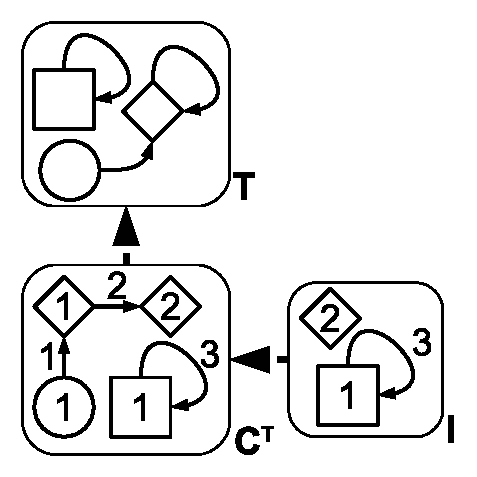
\includegraphics[scale=0.5]{images/process/unconditional-relation/core-graph}}}
    \caption{Core and initial graphs}\label{fig:process:unconditional-relation:core-graph}
  \end{subfigure}

  \begin{subfigure}[t]{.5\textwidth}
    \centerline{\fbox{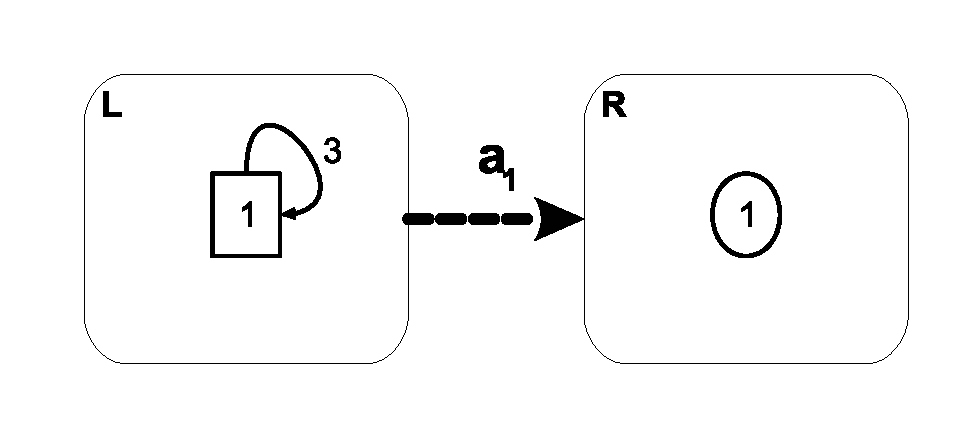
\includegraphics[scale=0.45]{images/process/unconditional-relation/a1}}}
    \caption{Action $a_1$}\label{fig:process:unconditional-relation:a1}
  \end{subfigure}%
  \begin{subfigure}[t]{.5\textwidth}
    \centerline{\fbox{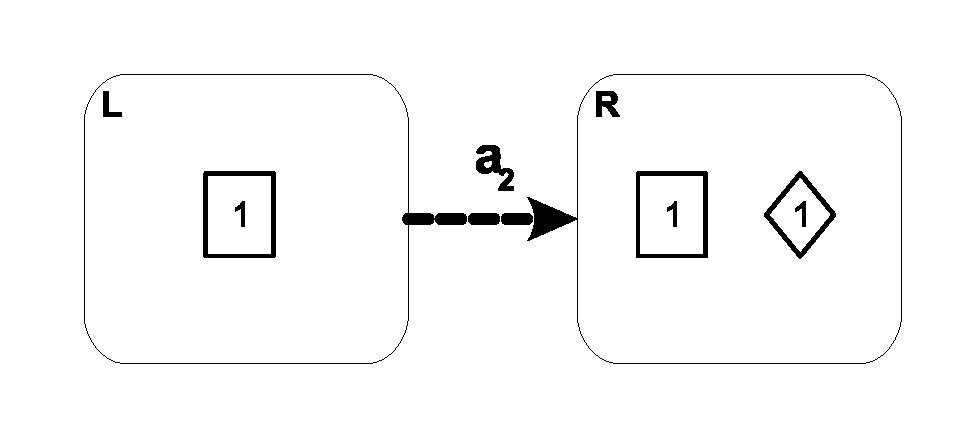
\includegraphics[scale=0.45]{images/process/unconditional-relation/a2}}}
    \caption{Action $a_2$}\label{fig:process:unconditional-relation:a2}
  \end{subfigure}

  \begin{subfigure}[t]{.5\textwidth}
    \centerline{\fbox{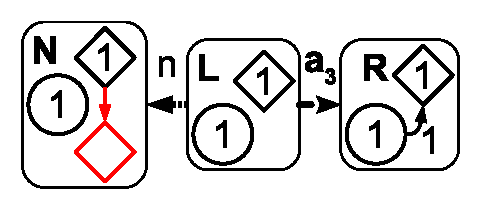
\includegraphics[scale=0.45]{images/process/unconditional-relation/a3}}}
    \caption{Action $a_3$}\label{fig:process:unconditional-relation:a3}
  \end{subfigure}%
  \begin{subfigure}[t]{.5\textwidth}
    \centerline{\fbox{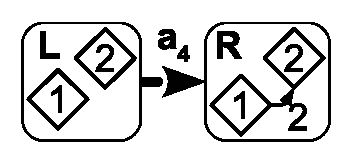
\includegraphics[scale=0.45]{images/process/unconditional-relation/a4}}}
    \caption{Action $a_4$}\label{fig:process:unconditional-relation:a4}
  \end{subfigure}
  \stepcounter{doubly-typed-grammar-counter}
  \caption{Strongly safe grammar GG\arabic{doubly-typed-grammar-counter}}\label{fig:process:unconditional-relation}
\end{figure}

\begin{definition}[Unconditional Causal Dependency Relation\footnote{Also called Produce-Use Relation.}]\label{def:unconditional-causal-dependency} Given \doublyTypedGraphGrammarCore{} a strongly safe graph grammar. Let $a_1, a_2 \in P$, $a_1 \ne a_2$, \mbox{$e_1, e_2 \in $ \coreGraph{}} and $e_1 \ne e_2$. Then: 

  \begin{enumerate}
    \item The action $a_2$ is \emph{directly causally dependent} on $a_1$, written $a_1 <_{pu} a_2$, iff \mbox{$\not\exists h_{21} : L_2 \rightarrow D_1$ s.t. \mbox{$d_1 \circ h_{21} = pre_2$}}, where the two squares are pushouts and $C^T_{|R_1L_2}$ ($C^T$ restricted to the joint image of $post_1$ and $pre_2$) satisfies the NACs for $a_2$ and $a_1^{-1}$.

\diagram{
   & & N_1^{-1} & & N_2 & & \\
      L_1 & K_1\ar[d]\ar[l]\ar[r] & R_1\ar[u]\ar[dr]_{post_1} & & L_2\ar[u]\ar@{.>}@/_1.1pc/[dlll]|{|}_<<<<{h_{21}}\ar[dl]^{pre_2} & K_2\ar[l]\ar[r]\ar[d] & R_2\\
       & D_1\ar@{^{(}->}[rr]_{d_1} & & C^T_{|R_1L_2} & & D_2\ar@{_{(}->}[ll]^{e_2} &}

   \item The \emph{causal dependency relation between actions} $\leq_{pu}$ of $P$ is the reflexive and transitive closure of the direct causal dependency.
   \item The element $e_2$ is \emph{directly causally dependent} on $e_1$, written $e_1 <_{pu} e_2$, iff there is an action $a_1 \in P$ such that $a_1$ deletes $e_1$ and creates $e_2$.
   \item The \emph{causal dependency relation between elements} $\leq_{pu}$ of $N(C^T) \cup E(C^T)$ is the reflexive and transitive closure of the direct causal dependency.
   \item The \emph{unconditional causal dependency relation} of a strongly safe grammar is defined as the transitive and reflexive closure of the union of both relations $\leq_{pu}$ for $P$ and $N(C^T) \cup E(C^T)$.
  \end{enumerate}
\end{definition}

\begin{example}[Unconditional Dependency Example]Figure~\ref{fig:process:unconditional-relation:dependency} \tinytodo{review the names of the graphs} shows a produce-use between the actions $a_2$ and $a_4$ of the strongly safe grammar depicted in Figure~\ref{fig:process:unconditional-relation}.

  This conflict occurs due to the fact that, besides both actions have valid graph transformations (they satisfy the rewriting conditions for the overlapping on $C^T$ restricted do the image of $post_2$ and $pre_4$ and none of them has any NACs), it is not possible to find a morphism from $L_4$ to $D_2$ satisfying the conditions on Definition~\ref{def:unconditional-causal-dependency}.

\begin{figure}[!ht]
  \centering
  \fbox{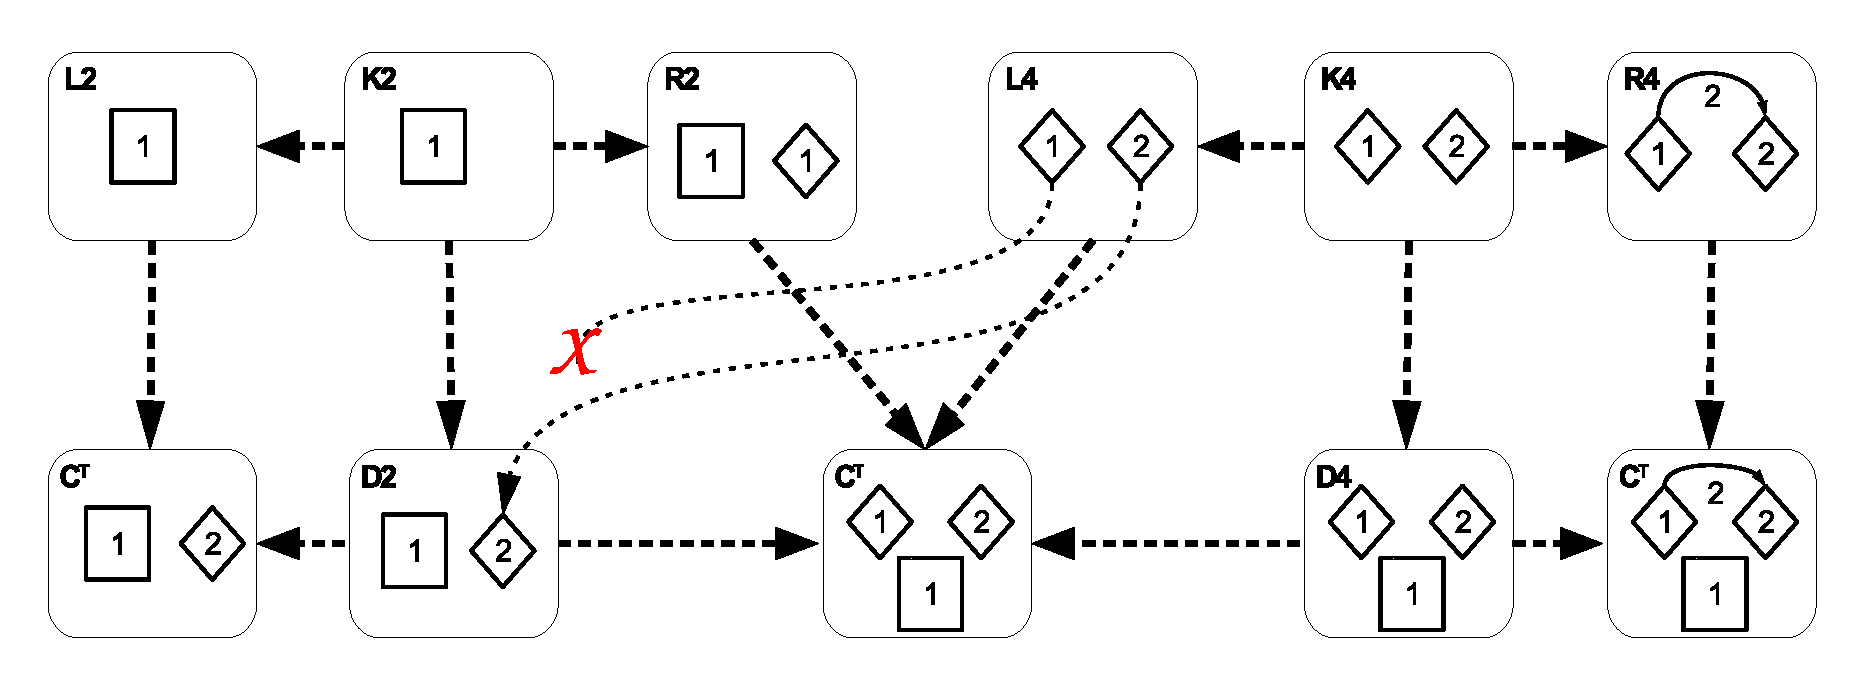
\includegraphics[scale=0.48]{images/process/unconditional-relation/dependency}}
  \caption{Unconditional causal dependency situation}\label{fig:process:unconditional-relation:dependency}
\end{figure}
\end{example}

Regarding both unconditional and conditional weak conflict relations, their definitions are based on the following intuition:

  \begin{intuition} An action $a_1$ is in \emph{weak} conflict with an action $a_2$ if either $a_1$ deletes something that is needed by $a_2$ to be applied (unconditional weak conflict) or creates something that is both forbidden by a NAC of $a_2$ and not deleted before the application of $a_2$ (conditional weak conflict). In both cases, we have that $a_2$ can not be applied once $a_1$ has been applied, in other words, $a_2$ can only be applied before $a_1$.
\end{intuition}

\begin{definition}[Unconditional Weak Conflict Relation\footnote{Also called Delete-Use Relation.}]\label{def:unconditional-conflict} Given \doublyTypedGraphGrammarCore{} a strongly safe graph grammar. Let $a_1, a_2 \in P$, $a_1 \ne a_2$, \mbox{$e_1, e_2 \in $ \coreGraph{}} and $e_1 \ne e_2$. Then: 

  \begin{enumerate}
    \item The action $a_1$ is in \emph{direct weak conflict} with $a_2$, written $a_2 <_{du} a_1$, iff \mbox{$\not\exists h_{21} : L_2 \rightarrow D_1$} s.t. \mbox{$d_1 \circ h_{21} = pre_2$}.

      \diagram{
          & & N_1 & & N_2 & & \\
        R_1 & K_1\ar[l]\ar[r]\ar[d] & L_1\ar[u]\ar[dr]_{pre_1} & & L_2\ar[u]\ar[dl]^{pre_2}\ar@{.>}@/_1.1pc/[dlll]|{|}_<<<<{h^{21}} & K_2\ar[l]\ar[r]\ar[d] & R_2\\
       & D_1\ar[rr]_{d_1} & & C^T_{|L_1L_2} & & D_2\ar[ll] &}
   \item The \emph{weak conflict relation between actions} $\leq_{du}$ of $P$ is the reflexive and transitive closure of the direct weak conflict.
   \item The element $e_2$ is \emph{in direct weak conflict} with $e_1$, written $e_2 <_{du} e_1$, iff there are actions $a_1$ and $a_2$ that respectively create $e_1$ and $e_2$ and $a_2 \leq_{du} a_1$.
   \item The \emph{weak conflict relation between elements} $\leq_{du}$ of $N(C^T) \cup E(C^T)$ is the reflexive and transitive closure of the direct weak conflict.
   \item The \emph{weak conflict relation} of a strongly safe grammar is defined by transitive and reflexive closure of the unions of relations $\leq_{du}$ for $P$ and $N(C^T) \cup E(C^T)$.

  \end{enumerate}
\end{definition}

\begin{example}[Unconditional Weak Conflict Example] Figure~\ref{fig:process:unconditional-relation:conflict} shows a delete-use between the actions $a_1$ and $a_2$ of the strongly safe grammar depicted in Figure~\ref{fig:process:unconditional-relation}.

  Again, both actions have valid graph transformations, now for the overlapping of $pre_1$ and $pre_2$ on $C^T$, but it is not possible to find a morphism from $L_2$ to $D_1$ satisfying the conditions on Definition~\ref{def:unconditional-conflict}.
\begin{figure}[!ht]
  \centering
  \fbox{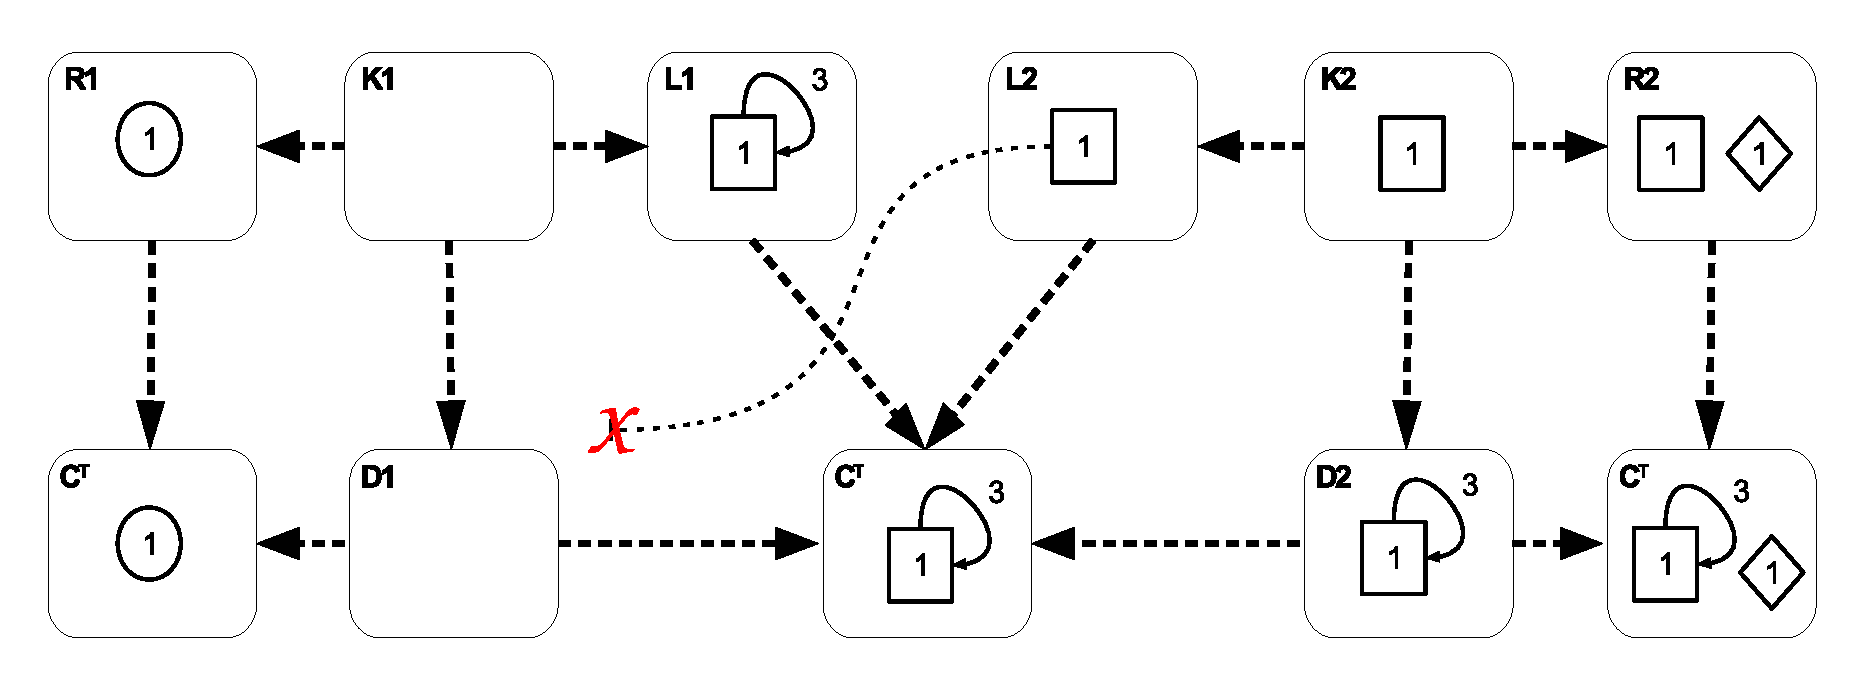
\includegraphics[scale=0.48]{images/process/unconditional-relation/conflict}}
  \caption{Unconditional weak conflict situation}\label{fig:process:unconditional-relation:conflict}
\end{figure}
\end{example}

\begin{definition}[Unconditional Occurrence Relation] Given \doublyTypedGraphGrammarCore{} a strongly safe graph grammar, let $\leq_{pu}$ and $\leq_{du}$ be the unconditional dependency and unconditional weak conflict relations of this grammar for $P \cup N(C^T) \cup E(C^T)$. Then the \emph{unconditional occurrence relation} of GG is the reflexive and transitive closure of \mbox{$\leq_{pu} \cup \leq_{du}$}.
\end{definition}

Similarly to the existential relation,~\cite{Ribeiro1996} proved that if this relation is a partial order, then it is possible to apply all actions of its underlying grammar in any total order that respects the partial order. Again, this condition is not sufficient if the rules may be equipped with NACs, as it was also shown to be equivalent to the existential relation.
